\section{Introduction} \label{introduction} 

Progress in some branches of
mathematics might be restricted by size of symbolic derivations that humans can
handle. Mathematicians can deal with expressions having dozens of
variables but would struggle to discover useful relations between hundreds or
thousands of variables. We will show how the task of finding equivalent
mathematical expressions can be automated. Our focus is on finding equivalent
mathematical formulas (i.e.~which give an identical numerical result
to the original expression),
but are faster to compute. The definition
of faster can be either (i) the number of operations or (ii) the computational time
for a particular hardware.

We propose a deterministic, grammar-based framework which discovers
relations between multi-variable polynomial expressions. First, we
construct an attribute grammar -- a context-free grammar extended to
contain set of attributes, introduced by Donald Knuth
\cite{knuth1968semantics}. To define the search space we use a set of
context-free grammar rules representing admissible operations. By
representing the cost of every operation as a synthesized attribute
(i.e. computed bottom-up from child node attributes) we can search for
formula with low time complexity. Through a linear combination of
grammar elements, we can find a solution to the desired
expressions. Finally, this computation solution can be further speed
up by use of standard techniques of optimization in compiler
domain. 

Example 1 shows our framework applied to a simple matrix expression:
\texttt{sum(sum(A*B))}, where \texttt{A} and \texttt{B} are matrices. Naively, this takes $O(n^3)$ to compute due to
the matrix multiply operation. The example outlines how our framework
can find an alternate way of computing {\em exactly} the same result,
but in $O(n^2)$ time.  

We demonstrate the flexibility of our technique by applying it to two
diverse problems in machine learning: 
\begin{enumerate}
\vspace{-2mm}
\item A Taylor-series approximation to the partition function of a
  binary RBM. We can produce a 6th order approximation which is
  computable in closed-form which takes $O(n^3)$ time (where $n$ is the
  number of visible \& hidden units). Naive evaluation of the Taylor-series
  approximation would require summing over the $2^N$ possible states.   
\item Closed-form computation of DropOut. DropOut \cite{Hinton12}
  involves the  stochastic deletion of outputs within a dense neural
  network layer at training time. For $n$ output units, the $2^n$
  possible deletion patterns are sampled indpeendently for each
  training sample. We use our framework to derive a closed-form
  expression that integrates out over all $2^n$ states.  
\end{enumerate}
\vspace{-2mm}

The main contribution of the paper is the introduction of a general
framework for discovering efficient closed-form expressions. Its
flexibility means can be used on a wide range of problems encountered
in math and AI, beyond those outlined above.

\framebox[3.27in][c]{\parbox{3.0in}{{\bf Example 1:}
\vspace{2mm}

We are given matrices $A \in \mathbb{R}^{n \times m}$, $B \in \mathbb{R}^{m \times k}$. We wish
 to compute \texttt{sum(sum(A*B))}, i.e.~: 
\vspace{1.5mm} \\ 
$\sum_{n,k} AB = \sum_{i = 1}^n \sum_{j = 1}^m \sum_{l = 1}^k A_{i, j} B_{j, l} $
\vspace{1.5mm} \\ 
which naively takes $O(nmk)$ time. Our framework is able to discover
an efficient version of the formula, that computes the same result in $O(n(k+m))$
time:
 \vspace{1mm} \\
%\begin{verbatim}
\texttt{	sum(sum(A .* repmat(sum(B, 2), [1, n])'))}
 \vspace{1mm} \\ 
Our framework has four distinct stages:
 \begin{enumerate}
\item An {\em attribute grammar} is defined (Section \ref{sec:grammars}).
\item The {\em grammar tree} is built (see Algorithm 1). This contains
  an exhaustive set of all valid compositions of expressions from the
  grammar. While slow, this only needs to be performed once for a
  given grammar, irrespecitve of the number of target expressions we
  wish to compute. The figure below shows two branches of the grammar
  tree.
\item Each leaf of this tree is checked to see if the result matches the
  target expression. This may require solving a linear system, if the
  target expression has multiple terms (see Section \ref{sec:linear}). The two leaves \texttt{L$_1$} and
  \texttt{L$_2$} shown in the tree produce the same result as the target
  expression. 
\item The computational complexity of the valid branches is then
  compared. The \texttt{L$_1$} branch is dominated by the
  \texttt{Matrix\_Multiply} operation which is $O(nkm)$. The
  \texttt{L$_2$} branch has several operations that take $O(nk)$ or
  $O(nm)$ time, so is preferred.
\end{enumerate}

Empirical tests indicate that our expression is indeed faster to
compute than the naive one (see Figure \ref{ab}).

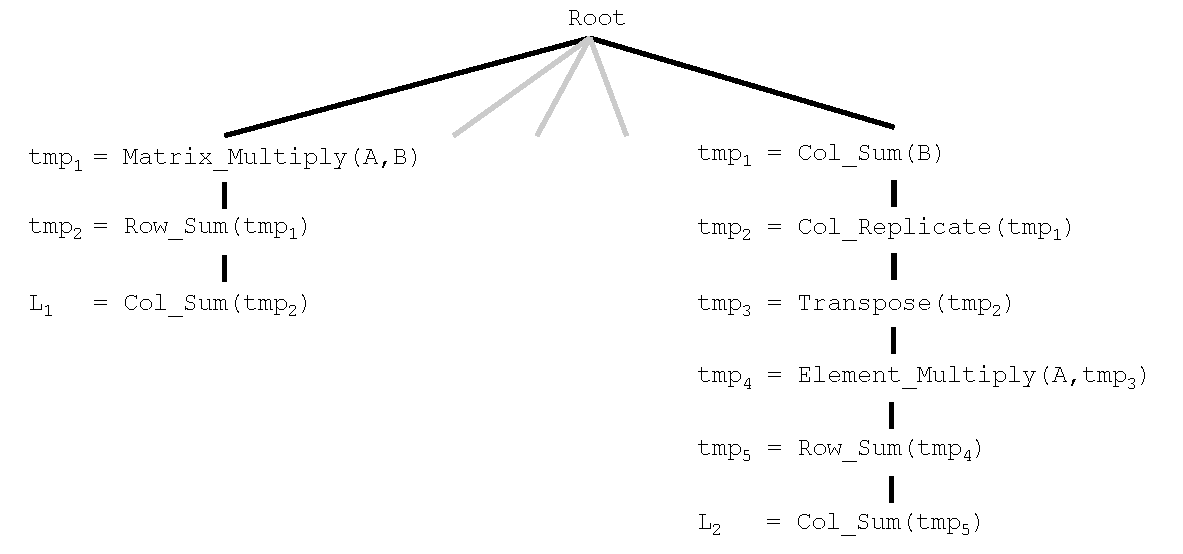
\includegraphics[scale=0.4]{img/toy_tree.pdf}
}}
%\end{verbatim}} 



% This
%violates the conventional wisdom that accurate computation of the
%partition function requires an exponential number of elements.


%Finally, we can regard the set of generated rules as a algebra with many operators 
%(grammar productions). 
%Goal of algorithm is to find shortest path to the target expression. 
%The brute force algorithm that we consider
%constructs the graph by advancing sequentially from smallest to largest degree.




